\chapter{The Curse of Dimensionality --- And How Humans Solve It}
\label{ch:curse-dim}

\epigraph{%
  In ten dimensions, the unit hypercube has $2^{10} = 1024$ corners.
  In a hundred, it has $2^{100} \approx 10^{30}$.
  The nervous system controls hundreds of dimensions every second.
}{}

\section{Classical Curse of Dimensionality}

The curse of dimensionality \cite{Bellman1961} states that the computational resources
needed to solve many problems grow \emph{exponentially} with the state dimension $n$:

\begin{definition}{The Curse of Dimensionality}{curse-def}
  For a control problem with state dimension $n$:
  \begin{itemize}
    \item \textbf{Grid-based methods} (dynamic programming): cost $\sim \mathcal{O}(N^n)$
          where $N$ is the grid resolution per dimension
    \item \textbf{Sample-based methods} (Monte Carlo, RL): sample complexity grows
          polynomially in $n$ but with large constants
    \item \textbf{Trajectory optimization} (DDP, collocation): cost $\sim \mathcal{O}(n^3 \cdot T)$
          per iteration --- the only scalable approach for deterministic systems
  \end{itemize}
\end{definition}

\begin{figure}[h]
\centering
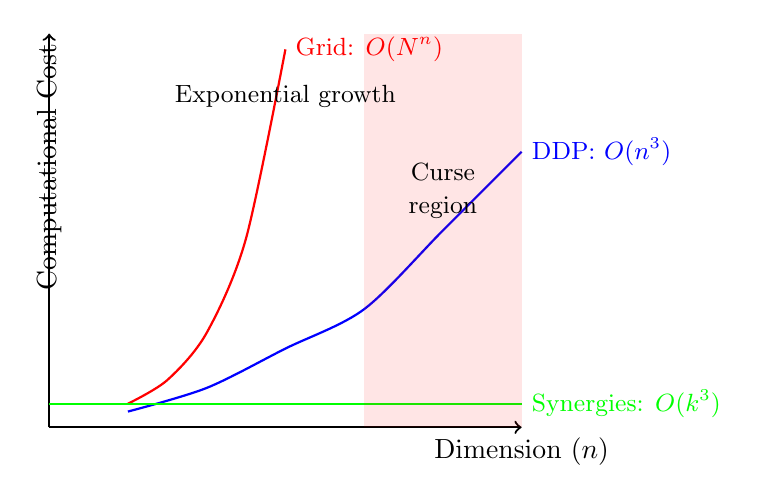
\begin{tikzpicture}[scale=1.0]
  % Axes
  \draw[->, thick] (0, 0) -- (6, 0) node[align=center, anchor=north] {Dimension ($n$)};
  \draw[->, thick] (0, 0) -- (0, 5) node[align=center, anchor=east, rotate=90] {Computational Cost};

  % Grid-based (exponential)
  \draw[red, thick, smooth] plot coordinates {
    (1, 0.3) (1.5, 0.6) (2, 1.2) (2.5, 2.4) (3, 4.8)
  } node[anchor=west] {\small Grid: $O(N^n)$};

  % DDP (cubic)
  \draw[blue, thick, smooth] plot coordinates {
    (1, 0.2) (2, 0.5) (3, 1.0) (4, 1.5) (5, 2.5) (6, 3.5)
  } node[anchor=west] {\small DDP: $O(n^3)$};

  % Synergy reduction (flat)
  \draw[green, thick] (0, 0.3) -- (6, 0.3) node[align=center, anchor=west] {\small Synergies: $O(k^3)$};

  % Shaded region (infeasible)
  \fill[red, opacity=0.1] (4, 5) -- (6, 5) -- (6, 0) -- (4, 0) -- cycle;
  \draw (5, 3) node[anchor=center, align=center] {\small Curse\\ \small region};

  \draw (3, 4.2) node[align=center, anchor=center, font=\small] {Exponential growth};
\end{tikzpicture}
\caption{The curse of dimensionality: computational cost grows exponentially with dimension
for grid-based methods, cubically for DDP, and remains constant when using synergy-based
dimensionality reduction (where $k \ll n$).}
\label{fig:ch2:curse-viz}
\end{figure}

\section{Biological Solutions}

Humans solve the dimensionality problem through five complementary mechanisms:

\subsection{1. Synergy-Based Compression}
As introduced in Chapter~4: $\bm{u}(t) = W \bm{c}(t)$ reduces $p$-dimensional muscle
space to $k$-dimensional synergy space, with $k/p \approx 4/400 = 1\%$.

\subsection{2. Hierarchical Decomposition}
Multi-level processing decomposes the global problem into independent subproblems.

\subsection{3. Passive Dynamics Exploitation}
The drift field $f(\state)$ does useful work. The controller only corrects deviations.
This reduces the effective control dimension (Volume~II, passive dynamics).

\subsection{4. Internal Models and Prediction}
Forward models predict consequences, enabling open-loop execution with sparse
feedback corrections (see Chapter~6).

\subsection{5. Task-Space Control}
Control in a low-dimensional task space rather than the full joint/muscle space.
The null space absorbs variability (UCM framework, Chapter~1).

\begin{lstlisting}[language=Python, caption={Computational cost comparison across methods.}]
import numpy as np

def computational_cost_table(n_dims: list[int]) -> None:
    """Print computational cost for different methods vs dimension."""
    print(f"{'n_dim':>6} {'Grid (N=10)':>15} {'DDP (T=100)':>15} "
          f"{'Synergy (k=5)':>15}")
    print("-" * 55)
    for n in n_dims:
        grid_cost = 10**n if n <= 10 else float('inf')
        ddp_cost = n**3 * 100
        synergy_cost = 5**3 * 100  # After reduction to k=5
        print(f"{n:>6d} {grid_cost:>15.0e} {ddp_cost:>15.0e} "
              f"{synergy_cost:>15.0e}")

computational_cost_table([2, 5, 10, 20, 50, 100, 200])
\end{lstlisting}

\section*{Exercises}

\begin{enumerate}
  \item \textbf{Scaling Analysis.}
        Using the computational cost table, determine the maximum state dimension for
        which grid-based dynamic programming is feasible (assuming $10^{12}$ FLOPS).

  \item \textbf{Synergy Efficiency.}
        If a motor task uses 100 muscles with 5 synergies, by what factor does the
        synergy decomposition reduce the dimensionality of the control problem?

  \item \textbf{(Programming.)} Implement DDP for a 2-DOF, 5-DOF, and 10-DOF chain.
        Measure computation time per iteration. Verify cubic scaling in state dimension.
\end{enumerate}
